\documentclass[ucs, notheorems, handout, 10pt]{beamer}

\usetheme[numbers,totalnumbers,compress, nologo]{Statmod}
%\usetheme{Madrid}
\usefonttheme[onlymath]{serif}
\setbeamertemplate{navigation symbols}{}

\mode<handout> {
	\usepackage{pgfpages}
	\setbeameroption{show notes}
	\pgfpagesuselayout{2 on 1}[a4paper, border shrink=5mm]
	\setbeamercolor{note page}{bg=white}
	\setbeamercolor{note title}{bg=gray!10}
	\setbeamercolor{note date}{fg=gray!10}
}

\usepackage[utf8x]{inputenc}
\usepackage[T2A]{fontenc}
\usepackage[russian]{babel}
\usepackage{tikz}
\usepackage{ragged2e}
\usepackage{amsmath,amssymb,amsthm,amscd,amsfonts}

\newtheorem{theorem}{Теорема}
\newtheorem{defenition}{Определение}

\title[Оценивание значимости выравнивания]{Задачи оценивания значимости выравнивания при помощи скрытых марковских моделей}

\author{Власенко Даниил Владимирович, гр.19.Б04-мм}

\institute[Санкт-Петербургский Государственный Университет]{%
	\small
	Санкт-Петербургский государственный университет\\
	Прикладная математика и информатика\\
	Вычислительная стохастика и статистические модели\\
	\vspace{1.25cm}
	Отчет по производственной практике}

\date[Зачет]{Санкт-Петербург, 2022}

\subject{Talks}


\begin{document}
	
	\begin{frame}[plain]
		\titlepage
		
		\note{Научный руководитель  к.ф.-м.н., Коробейников А.И.,\\
			кафедра статистического моделирования}
	\end{frame}
	
	\begin{frame}{Введение}
		\begin{defenition}
			Выравнивание последовательностей  "--- размещение двух или более последовательностей друг под другом таким образом, чтобы было легче увидеть их схожие участки.
		\end{defenition}
		
		\begin{figure}
			\begin{tabular}{cccccccc}
				A&C&E&A&A&F&A&E\\
				C&E&A&F&D&C&E&\\
			\end{tabular}
		\end{figure}
		\begin{figure}
			\begin{tabular}{ccccccccc}
				A&C&E&A&A&F&A&—&E\\
				—&C&E&A&—&F&D&C&E\\
			\end{tabular}
			\caption{Последовательности до и после выравнивания.} \label{fg:1}
		\end{figure}
		
		\begin{defenition}
			Значимость выравнивания "--- действительное число $s$, отражающее сходство последовательностей.
		\end{defenition}
		
		\note{
			Последовательность длины $L$ "--- строка $D$ состоящая из $L$ символов алфавита $\Sigma$. Выравнивание последовательностей  "--- размещение двух или более последовательностей друг под другом таким образом, чтобы было легче увидеть их схожие участки. Например, даны последовательности ACEAAFAE и CEAFDCE, если расположить их друг под другом, то не будет ни одного совпадения соответствующих символов, но если вставить пропуск восьмого символа в первой последовательности и пропуски первого и пятого символов во второй последовательности, то мы получим 5 совпадений.
			
			Значимость выравнивания "--- действительное число $s$, отражающее сходство последовательностей. Способом вычисления значимости выравнивания $s$ может быть, например, увеличение значимости на 1 при совпадении символов, стоящих друг под другом, и уменьшение на $\frac{1}{2}$ при несовпадении. Тогда значимость $s$ приведенного выше выравнивания будет равна 3. Способ вычисления значимости выравнивания выбирается исходя из целей и вида выравнивания. 
		}
	\end{frame}

	\begin{frame}{Введение}
		\begin{defenition}
			Выравнивание последовательностей  "--- размещение двух или более последовательностей друг под другом таким образом, чтобы было легче увидеть их схожие участки.
		\end{defenition}
		
		\begin{figure}
			\begin{tabular}{cccccccc}
				A&C&E&A&A&F&A&E\\
				C&E&A&F&D&C&E&\\
			\end{tabular}
		\end{figure}
		\begin{figure}
			\begin{tabular}{ccccccccc}
				A&C&E&A&A&F&A&—&E\\
				—&C&E&A&—&F&D&C&E\\
			\end{tabular}
			\caption{Последовательности до и после выравнивания.} \label{fg:1}
		\end{figure}
		
		\begin{defenition}
			Значимость выравнивания "--- действительное число $s$, отражающее сходство последовательностей.
		\end{defenition}
		
		\note{						
			Сходство последовательностей может отражать функциональные, структурные или эволюционные взаимосвязи объектов, которые описывают эти последовательности. Таким образом вычисление значимости выравнивания последовательностей может быть полезно в задаче определения степени родства биологических организмов путем сравнения их ДНК или РНК, нуклеотидных последовательностей, задаче анализа свойств белков, аминокислотных последовательностей, задаче распознавания речи человека или письменного языка и многих других приложениях.
			
			На слайде приведен пример попарного выравнивания двух строк, но если сходство последовательностей слабое, то через такое выравнивание может не выйти идентифицировать взаимосвязь описываемых последовательностями объектов. Однако сравнение сразу трех и более последовательностей может позволить выявить эту взаимосвязь, такое выравнивание называется множественным. Проводить множественное выравнивание стандартными методами динамического программирования для попарного выравнивания вычислительно неэффективно, но оказывается, что аппарат скрытых марковских моделей (СММ) позволяет эффективно решать эту задачу. 
		}
	\end{frame}

	\begin{frame}{Введение}
		\begin{itemize}
			\item достаточно ли высокая значимость, чтобы считать последовательность не шумом, или шум мог добиться такой значимости.
			\item достаточно ли низкая значимость, чтобы считать последовательность шумом, или не шум мог получить такую значимость. 
		\end{itemize}
		
		\begin{defenition}
			Ложноположительная вероятность значимости $s$ "--- это вероятность того, что шум получит значимость равную или выше $s$. 
		\end{defenition}
		
		\note{	
			СММ будут описаны далее, пока что зададимся следующим вопросом. Если есть множество последовательностей, описывающих взаимосвязанные объекты, имеется еще одна последовательность и была посчитана значимость выравнивания этой последовательности ко всему множеству каким-либо способом, то
			\begin{itemize}
				\item достаточно ли высокая эта значимость, чтобы считать объект, описываемый последовательностью, родственным к объектам, описываемым множеством, или шум, т.е. случайная последовательность, мог добиться такой значимости.
				\item достаточно ли низкая эта значимость, чтобы считать объект описываемый последовательностью, не родственным к объектам, описываемым множеством, или сигнал, т.е. последовательность, описывающая взаимосвязанный с множеством объект, мог получить такую значимость. 
			\end{itemize}
			Ложноположительная вероятность значимости $s$ "--- это вероятность того, что шум получит значимость равную или выше $s$. 
			
			Далее будет описаны метод, который позволяет эффективно вычислять введенный термин.								
		}
	\end{frame}

	\begin{frame}{Обозначения и известные результаты}
		\begin{defenition}
			Пусть $X_{n}$ и $Y_{n}$ дискретные стохастические процессы, $n \geq 1$. Пара $(X_{n}, Y_{n})$ называется скрытой марковской моделью, если
			\begin{itemize}
				\item $X_{n}$~--- марковский процесс, поведение которого напрямую не наблюдается ("скрытый");
				\item $\mathsf{P}(Y_{n} = y_{n}|X_{1} = x_{1},\dots, X_{n} = x_{n}) = \mathsf{P}(Y_{n}|X_{n}=x_{n})$ для любого $n \geq 1$, где $x_{1},\dots,x_{n}$~--- значения, принимаемые процессом  $X_{n}$ (\textbf{состояния модели}), $ y_{n}$~--- значение, принимаемое процессом $Y_{n}$ (\textbf{наблюдаемый символ модели}).
			\end{itemize}
		\end{defenition}
		
		\note{						
			Сначала опишем модели, затем алгоритмы, которые используются для манипуляции ими.
			
			Метод предполагает, что даны профильная СММ, с помощью которой будут оцениваться последовательности, и фоновая модель $B$, которая будет описывать шум.
			
			\begin{defenition}
				Пусть $X_{n}$ и $Y_{n}$ дискретные стохастические процессы, $n \geq 1$. Пара $(X_{n}, Y_{n})$ называется скрытой марковской моделью, если
				\begin{itemize}
					\item $X_{n}$~--- марковский процесс, поведение которого напрямую не наблюдается ("скрытый");
					\item $P(Y_{n} = y_{n}|X_{1} = x_{1},\dots, X_{n} = x_{n}) = P(Y_{n}|X_{n}=x_{n})$ для любого $n \geq 1$, где $x_{1},\dots,x_{n}$~--- значения, принимаемые процессом  $X_{n}$ (\textbf{состояния модели}), $ y_{n}$~--- значение, принимаемое процессом $Y_{n}$ (\textbf{наблюдаемый символ модели}).
				\end{itemize}
			\end{defenition}
		}
	\end{frame}

	\begin{frame}{Обозначения и известные результаты}
		\begin{figure}[h]
			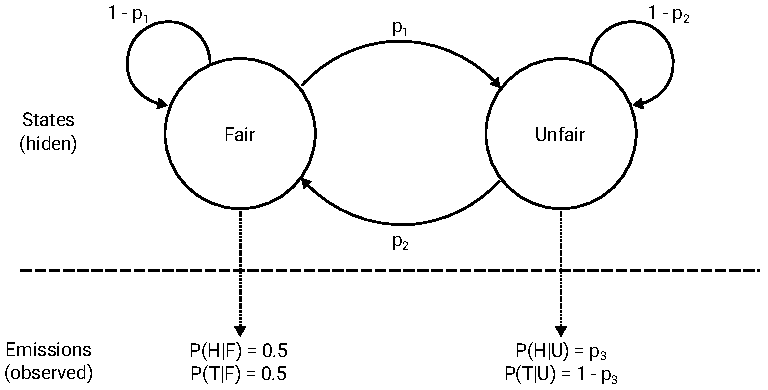
\includegraphics[width=10cm]{../../report/figure1}
			\caption{Простая скрытая марковская модель.} \label{fg:2}
		\end{figure}
		
		\note{						
			Примером простой СММ может быть модель, изображенная на слайде и описывающая подбрасывание двух монет. Пусть между наблюдателем и человеком с монетами стоит ширма, которая позволяет наблюдателю видеть только пол, куда падают монеты. Пусть есть две монеты: одна "--- честная монета, вторая "--- нечестная монета с перевесом в одну из сторон. Пусть человек с монетами с некоторой вероятностью либо подбрасывает монету, которую он бросил в прошлый раз, либо меняет монеты и бросает новую. При этом наблюдатель не знает, какая монета используется в конкретный момент времени, так как он не видит рук бросающего монеты и не может отличить одну монету от другой по их внешнему виду, он видит только последовательность результатов бросков.
		}
	\end{frame}
	
	\begin{frame}{Обозначения и известные результаты}
		\begin{figure}[h]
			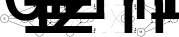
\includegraphics[width=11cm]{../../report/figure2}
			\caption{Профильная скрытая марковская модель.}  \label{fg:3}
		\end{figure}
				
		\note{
			Профильная СММ "--- это СММ со специальной линейной архитектурой состояний, которая позволяет выравнивать последовательность к множеству последовательностей.						
			
			Если для удобства реализации алгоритмов добавить специальное \textit{начальное} и специальное \textit{конечное} состояния, в которых профильная СММ начинает и заканчивает работу и не испускает наблюдаемых символов, как показано на слайде, тогда \textit{путь} $\pi$ в профильной СММ начинается в начальном состоянии, заканчивается в конечном состоянии и проходит от состояния к состоянию, испуская в каждом состоянии наблюдаемый символ, то есть мы считаем, что путь $\pi$ включает в себя и состояния, и наблюдаемые символы. \textit{Последовательность} $D$, связанная с путем $\pi$ "--- последовательность наблюдаемых символов, которая была получена в результате прохода профильной СММ пути $\pi$.
		}
	\end{frame}

	\begin{frame}{Обозначения и известные результаты}
		\begin{defenition}
			\textit{Вероятность последовательности} $D$ может интерпретироваться и считаться по-разному "--- алгоритмом \textit{Витерби} или \textit{Форвард} алгоритмом.
		\end{defenition}
		
		\begin{equation*}
			s_{max}(D) = \underset{\pi \in \pi_{D}}{max}(s(\pi)); \label{eq:1}
		\end{equation*}
		
		\begin{equation*}
			s_{fw}(D) = \sum_{\pi \in \pi_{D}}s(\pi); \label{eq:2}
		\end{equation*}
		
		\begin{equation*}
			Z(D, T)	= \sum_{\pi \in \pi_{D}}s(\pi)^{\frac{1}{T}}. \label{eq:3}
		\end{equation*}
		
		\note{
			\textit{Вероятность пути} $s(\pi)$ "--- произведение всех переходных вероятностей от состояний к состоянию и вероятностей наблюдаемых символов, которые излучаются в каждом состоянии, кроме начального и конечного, на протяжении всего пути $\pi$. 
			
			\textit{Вероятность последовательности} $D$ может интерпретироваться и считаться по-разному "--- алгоритмом \textit{Витерби} или \textit{Форвард} алгоритмом.
			
			Вероятность Витерби $s_{max}(D)$ последовательности $D$ "--- это максимальная вероятность последовательности $D$ среди всех путей $\pi$, которые могли бы ее испустить:
			\begin{equation}
				s_{max}(D) = \underset{\pi \in \pi_{D}}{max}(s(\pi)),
			\end{equation}
			Несмотря на большое количество возможных путей, которые могли бы испустить последовательность $D$, алгоритм Витерби позволяет эффективно решать эту задачу.
			
			Форвард вероятность $s_{fw}(D)$ последовательности $D$ "--- это общая вероятность того, что в результате работы СММ будет получена последовательность $D$:
			\begin{equation}
				s_{fw}(D) = \sum_{\pi \in \pi_{D}}s(\pi).
			\end{equation}			
		}
	\end{frame}

	\begin{frame}{Обозначения и известные результаты}
		\begin{defenition}
			\textit{Вероятность последовательности} $D$ может интерпретироваться и считаться по-разному "--- алгоритмом \textit{Витерби} или \textit{Форвард} алгоритмом.
		\end{defenition}
		
		\begin{equation*}
			s_{max}(D) = \underset{\pi \in \pi_{D}}{max}(s(\pi)); \label{eq:1}
		\end{equation*}
		
		\begin{equation*}
			s_{fw}(D) = \sum_{\pi \in \pi_{D}}s(\pi); \label{eq:2}
		\end{equation*}
		
		\begin{equation*}
			Z(D, T)	= \sum_{\pi \in \pi_{D}}s(\pi)^{\frac{1}{T}}. \label{eq:3}
		\end{equation*}
		
		\note{			
			Форвард алгоритм работает за то же время, что и алгоритм Витерби.
			
			Третий способ оценивать последовательности, позволяющий уменьшить дисперсию дальнейших вычислений оценки ложноположительной вероятности значимости, заключается в том, что каждая вероятность перехода из одного состояния в другое и вероятность излучения символа состоянием будут возводится в степень $\frac{1}{T}$, где $T \in (0; +\infty)$. При этом логика вычислений остается та же, то есть $s(\pi)^{\frac{1}{T}}$ и $s(D)^{\frac{1}{T}}$ будут вычисляться как вероятность произведения независимых событий и как сумма непересекающихся событий соответственно, хотя они уже могут не являться вероятностями (Например, сумма всех $s(\pi)^\frac{1}{T}$ не обязательно равна единице):
			\begin{equation}
				Z(D, T)	= \sum_{\pi \in \pi_{D}}s(\pi)^{\frac{1}{T}}.
			\end{equation}		
			Функция $Z(D, T)$ называется статистической суммой и вычисляется через модификацию Форвард алгоритма. Параметра $T$ подбирается экспериментально под конкретную интересующую значимость выравнивания.
		}
	\end{frame}

	\begin{frame}{Обозначения и известные результаты}
		Мы предполагаем наличие простой фоновой модели $B$ для последовательностей длины $L$ такой, что все $L$ символьных позиций независимы и одинаково распределены в соответствии с некоторым распределением $\mathsf{P}(d|B)$, где $d$ отражает возможный наблюдаемый символ:
		\begin{equation*}
			\mathsf{P}(D|B) = \prod_{i=1}^{L}\mathsf{P}(d_{i}|B), \label{eq:4}
		\end{equation*}
		где $d_{i}$ "--- это $i$-ый наблюдаемый символ последовательности $D$.
		
		\note{
			Мы предполагаем наличие простой фоновой модели $B$ для последовательностей длины $L$ такой, что все $L$ символьных позиций независимы и одинаково распределены в соответствии с некоторым распределением $\mathsf{P}(d|B)$, где $d$ отражает возможный наблюдаемый символ:
			\begin{equation*}
				\mathsf{P}(D|B) = \prod_{i=1}^{L}\mathsf{P}(d_{i}|B), \label{eq:4}
			\end{equation*}
			где $d_{i}$ "--- это $i$-ый наблюдаемый символ последовательности $D$.
		}
	\end{frame}

	\begin{frame}{Обозначения и известные результаты}
		\begin{defenition}
			Ложноположительная вероятность значимости $s_{0}$ для строк длины $L$:	
			\begin{equation}
				fpr(s_{0}) =  \sum_{D \in D_{L}} \mathsf{P}(D|B) \Theta(s(D) \geq s_{0}), \label{eq:5}
			\end{equation}
			где $\mathsf{P}(D|B)$ "--- условная вероятность последовательности $D$, описываемая фоновой моделью, $s(D)$ "--- вероятность последовательности $D$, считаемая профильной СММ, и
			\[
			\Theta(s(D) \geq s_{0}) = 
			\begin{cases}
				1, & s(D) \geq s_{0}\\
				0, & s(D) < s_{0}
			\end{cases}.
			\]
		\end{defenition}	
			
		\note{
			Вероятность последовательности $D$ длины $L$ сравнивается с остальными последовательностями той же длины. Определим ложноположительную вероятность значимости:
			\begin{equation}
				fpr(s_{0}) =  \sum_{D \in D_{L}} Pr(D|B) \Theta(s(D) \geq s_{0}),
			\end{equation}
			где $Pr(D|B)$ "--- условная вероятность последовательности $D$, описываемая фоновой моделью, $s(D)$ "--- вероятность последовательности $D$, считаемая профильной СММ, и
			\[
			\Theta(s(D) \geq s_{0}) = 
			\begin{cases}
				1, & s(D) \geq s_{0}\\
				0, & s(D) < s_{0}
			\end{cases}.
			\]
			То есть $fpr(s_{0})$ "--- это вероятность того, что шум достигнет или превзойдет значимость $s_{0}$. В определении $fpr(s_{0})$ вероятность $D$ отмечена как $s(D)$, потому что способ оценки последовательности может выбираться относительно интересующего приложения, подходит $s(D) = s_{max}(D)$ и $s(D) = s_{fw}(D)$.
		}
	\end{frame}

	\begin{frame}{Обозначения и известные результаты}
		Вычисление $fpr(s_{0})$ через формулу \eqref{eq:5} обычно неосуществимо, значение $fpr(s_{0})$ может быть оценено через выборку по значимости. 
		
		\vspace{0.5cm}
		
		Пусть $\mathsf{P}(D|T)$ "--- это условная вероятность строки $D$ относительно некоторой модели строк длины $L$ параметризованной значением $T$. Тогда можно переписать $fpr(s_{0})$:		
		
		\begin{equation*}
			fpr(s_{0}) = \sum_{D \in D_{L}} \mathsf{P}(D|T) f(D,s_{0}), \label{eq:6}
		\end{equation*}
		где
		\begin{equation}
			f(D,s_{0}) = \frac{\mathsf{P}(D|B) \Theta(s(D) \geq s_{0})}{\mathsf{P}(D|T)}. \label{eq:7}
		\end{equation}		
		
		\note{
			Так как вычисление $fpr(s_{0})$ через формулу 5 обычно неосуществимо, значение $fpr(s_{0})$ может быть оценено через выборку по значимости, то есть через моделирование строк в соответствии с фоновой моделью $B$ и оценивание значения $fpr(s_{0})$ долей тех из них, что достигают значимости $s_{0}$.
			
			Построим распределение, относительно которого будем моделировать строки. Пусть $P(D|T)$ "--- это условная вероятность строки $D$ относительно некоторой модели строк длины $L$ параметризованной значением $T$. Тогда можно переписать $fpr(s_{0})$:
			\begin{equation}
				fpr(s_{0}) = \sum_{D \in D_{L}} Pr(D|T) f(D,s_{0}),
			\end{equation}
			где
			\begin{equation}
				f(D,s_{0}) = \frac{Pr(D|B) \Theta(s(D) \geq s_{0})}{Pr(D|T)}.
			\end{equation}
			Мы можем оценить значение $fpr(s_{0})$ через моделирование последовательностей в соответствии с этой альтернативной моделью и подсчет среднего значения $f(D,s_{0})$. Этот подход и называется \textit{выборкой по значимости}, он полезен, потому что если правильно подобрать альтернативную модель, то удастся уменьшить дисперсию оценки $fpr(s_{0})$.
		}
	\end{frame}

	\begin{frame}{Обозначения и известные результаты}
		Определим модель, используемую для выборки по важности параметризованную $T$:		
		
		\begin{equation*}
			\mathsf{P}(D|T) = \frac{\mathsf{P}(D|B)Z(D,T)}{Z(T)}, \label{eq:8}
		\end{equation*}							
		где 
		\begin{equation*}
			Z(T) = \sum_{D \in D_{L}}\mathsf{P}(D|B)Z(D,T). \label{eq:9}
		\end{equation*}
		Подставив определение $\mathsf{P}(D,T)$ в уравнение \eqref{eq:7} получим
		\begin{equation*}
			f(D,s_{0}) = \frac{Z(T)\Theta(s(D) \geq s_{0})}{Z(D,T)}. \label{eq:10}
		\end{equation*}	
		
		\note{
			Определим модель, используемую для выборки по важности параметризованную $T$ следующим образом:
			\begin{equation}
				Pr(D|T) = \frac{P(D|B)Z(D,T)}{Z(T)},
			\end{equation}							
			где 
			\begin{equation}
				Z(T) = \sum_{D \in D_{L}}Pr(D|B)Z(D,T).
			\end{equation}	
			Подставив определение $Pr(D,T)$ в уравнение 7 получим 
			\begin{equation}
				f(D,s_{0}) = \frac{Z(T)\Theta(s(D) \geq s_{0})}{Z(D,T)}.
			\end{equation}	
			
			В итоге мы хотим смоделировать последовательности в соответствии с распределением $Pr(D|T)$, вычислить $f(D, s_{0})$ для каждой последовательности и использовать среднее этих значений как оценку $fpr(s_{0})$. 
			
			Опуская подробности того как устроены моделирование, построенное на модификациях классических алгоритмов, связанных с HMM, и метод подбора параметра $T$, перейдем к полученным результатам.
		}
	\end{frame}
	
	\begin{frame}{Полученные результаты}
		Вычислим оценку $\widehat{fpr}(s_{0})$ для строк длины $L=100$, состоящих из 5 символов, и доверительные интервалы уровня $\gamma = 0.99$:		
		\begin{table}
			\caption{Результаты.} \label{tb:1}
			\begin{tabular}{cccc}
				$s_{0}$&T&$\widehat{fpr}(s_{0})$&$[c_{1}(\gamma);c_{2}(\gamma)]$  \\ \hline
				$10^{-85}$&7&0.0000000183&[0.0; 0.00066349] \\
				$10^{-90}$&7&0.003175&[0.001884; 0.004779] \\ 
				$10^{-100}$&7&0.615709&[0.597540 0.622677] \\
			\end{tabular}
		\end{table}	
		
		\note{
			Вычислим оценку $\widehat{fpr}(s_{0})$ для строк длины $L=100$ и доверительные интервалы уровня $\gamma = 0.99$:
			\begin{center}
				\begin{tabular}{cccc}
					$s_{0}$&T&$\widehat{fpr}(s_{0})$&$[c_{1}(\gamma);c_{2}(\gamma)]$  \\ \hline
					$10^{-85}$&7&0.0000000183&[0.0; 0.00066349] \\
					$10^{-90}$&7&0.003175&[0.001884; 0.004779] \\ 
					$10^{-100}$&7&0.615709&[0.597540 0.622677] \\
				\end{tabular}
			\end{center}
			Вычисление $fpr(s_{0})$ перебором привело бы к перебору $5^{100}$ строк, что неосуществимо, если бы мы вычисляли перебором всех строк длины $L$.
		}
	\end{frame}
	
	\begin{frame}{Заключение}
		\begin{itemize}
			\item Была изучена тема алгоритмов парного и множественного выравнивания последовательностей и тема СММ и алгоритмов взаимодействия с ними.
			\item Был реализован алгоритм, позволяющий эффективно вычислять оценку ${fpr}(s_{0})$.
			\item Предстоит подробно верифицировать реализованный алгоритм и сравнить его с имеющимися методами вычисления оценки ${fpr}(s_{0})$.
		\end{itemize}
		
		\note{
			\begin{itemize}
				\item Была изучена тема алгоритмов парного и множественного выравнивания последовательностей и тема СММ и алгоритмов взаимодействия с ними.
				\item Был реализован алгоритм, позволяющий эффективно вычислять оценку ${fpr}(s_{0})$.
				\item Предстоит подробно верифицировать реализованный алгоритм и сравнить его с имеющимися методами вычисления оценки ${fpr}(s_{0})$.
			\end{itemize}
		}
	\end{frame}
	
	\begin{frame}{Список литературы}
		\nocite{Newberg2009}
		\nocite{Compeau2015}
		\nocite{Compeau2015a}
		\nocite{Dugad1996}		
		\bibliographystyle{../../report/ugost2008mod}
		\bibliography{../../report/references}   
		
		\note{
			На данном слайде представлен список основных источников, используемых в моей работе.
		}
	\end{frame}
	
\end{document}
